\section{GIT vs. SVN}
%
\subsection{R�ckblick zu SVN}
\begin{frame}
  \frametitle{R�ckblick zu SVN}
  \tableofcontents[currentsection,currentsubsection]
\end{frame}
\begin{frame}
  \frametitle{R�ckblick zu SVN}
  \begin{itemize}
    \item Repository auf zentralem Server einrichten
    \item<2->Arbeitskopie auschecken
      \begin{itemize}
        \item<3->Warten
      \end{itemize}
    \item<4->Dateien zur Versionierung hinzuf�gen
      \begin{itemize}
        \item<5->Warten
      \end{itemize}
    \item<6->Commit
      \begin{itemize}
        \item<7->Warten
      \end{itemize}
  \end{itemize}
\end{frame}
\begin{frame}
  \frametitle{Workflow SVN}
  \begin{center}
    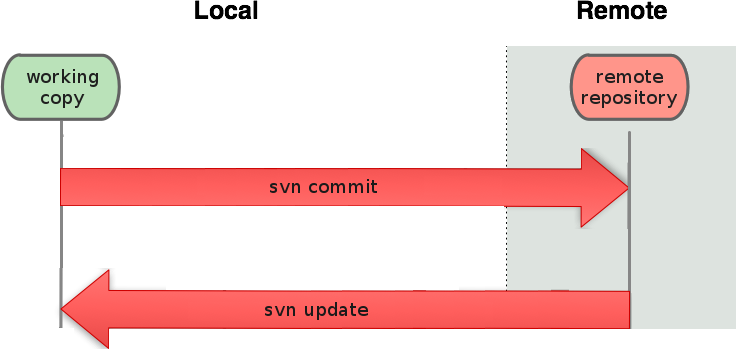
\includegraphics[width=0.95\textwidth]{images/local-remote-workflow-svn.png}
  \end{center}
\end{frame}
%
\subsection{Workflow mit GIT}
\begin{frame}
  \frametitle{Workflow mit GIT}
  \tableofcontents[currentsection,currentsubsection]
\end{frame}
\begin{frame}[fragile]
  \frametitle{Workflow mit GIT}
  \begin{itemize}
    \item Repository erstellen $\Leftrightarrow$ Arbeitskopie auschecken
      \begin{minted}[gobble=8]{sh}
        $ git init
      \end{minted}
    \item<2->Optional: Erzeugen einer \texttt{.gitignore}-Datei
    \item<3->Optional: Hinzuf�gen von Remotes
      \begin{minted}[gobble=8]{sh}
        $ git remote add origin git@thisdone.de:my_project.git
      \end{minted}
    \item<4->Dateien und �nderungen hinzuf�gen:
      \begin{minted}[gobble=8]{sh}
        $ git add .
      \end{minted}
    \item<5->Commit:
      \begin{minted}[gobble=8]{sh}
        $ git commit -m "Commit message"
      \end{minted}
    \item<6->Optional: Push auf Remote
      \begin{minted}[gobble=8]{sh}
        $ git push origin master
      \end{minted}
    \item<7->Hilfe f�r fast alle Kommandos: \texttt{git help <command>}
  \end{itemize}
\end{frame}
\begin{frame}
  \frametitle{Workflow mit GIT}
  \begin{center}
    \vspace{-7mm}
    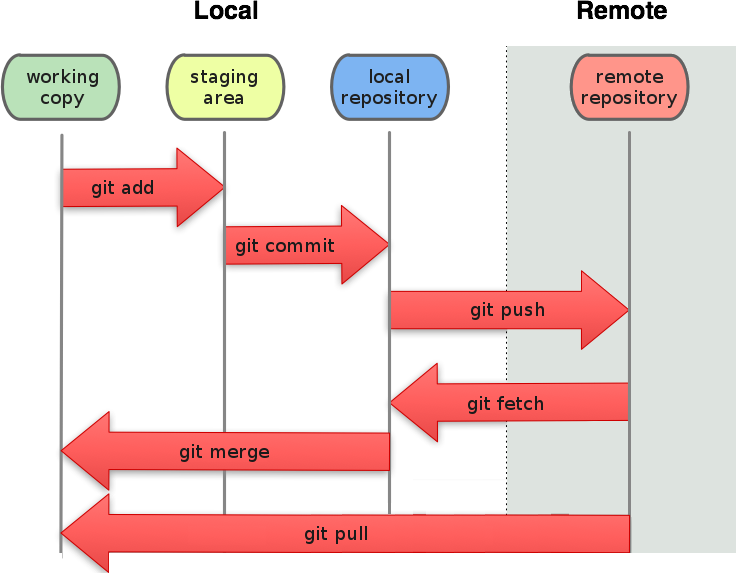
\includegraphics[height=.75\textheight]{images/local-remote-workflow-git.png}
  \end{center}
\end{frame}
%
\subsection{Tabellarischer Vergleich}
\begin{frame}
  \frametitle{Tabellarischer Vergleich}
  \tableofcontents[currentsection,currentsubsection]
\end{frame}
\begin{frame}
  \frametitle{Repositories \& Arbeitskopien}
  \begin{center}
    \begin{tabular}{|l|l|l|}
      \hline
      \textbf{Aktion} & \textbf{GIT} & \textbf{SVN} \\ \hline 
      \multirow{2}{*}{Erzeugen} & \texttt{cd <repo>} & \texttt{svnadmin create <repo>} \\
                                           & \texttt{git init .} & \texttt{svn checkout file://repo} \\ \hline
      Klonen & \texttt{git clone <url>} & \texttt{svn checkout <url>} \\ \hline
      Status & \texttt{git status} & \texttt{svn status} \\ \hline
    \end{tabular}
  \end{center}
\end{frame}
\begin{frame}
  \frametitle{Dateien \& Commits}
  \begin{center}
    \begin{tabular}{|l|l|l|}
      \hline
      \textbf{Aktion} & \textbf{GIT} & \textbf{SVN} \\ \hline
      Dateien hinzuf�gen & \texttt{git add <path>} & \texttt{svn add <path>} \\ \hline
      Dateien entfernen & \texttt{git rm <path>} & \texttt{svn rm <path>} \\ \hline
      Dateien verschieben & \texttt{git mv <path>} & \texttt{svn mv <path>} \\ \hline
    �nderungen hinzuf�gen & \texttt{git add <path>} & \texttt{???} \\ \hline
    Commit der �nderungen & \texttt{git commit} & \texttt{???} \\ \hline
  Commit aller �nderungen & \texttt{git commit -a} & \texttt{svn commit} \\ \hline
    \end{tabular}
  \end{center}
\end{frame}
\begin{frame}
  \frametitle{Remotes \& Branches}
  \begin{center}
    \begin{tabular}{|l|l|l|}
      \hline
      \textbf{Aktion} & \textbf{GIT} & \textbf{SVN} \\ \hline
      Commits auf Remote & \texttt{git push} & \texttt{svn commit} \\ \hline
      Commits von Remote & \texttt{git fetch} & \texttt{???} \\ \hline
      Commits von Remote mergen & \texttt{git pull} & \texttt{svn update} \\ \hline
      Branch erzeugen\footnote{Branch Kommandos funktionieren f�r Tags analog} & \texttt{git branch <name>} & \texttt{-} \\ \hline
      In Branch wechseln & \texttt{git checkout <name>} & \texttt{-} \\ \hline
      Branch mergen & \texttt{git merge <name>} & \texttt{-} \\ \hline
    \end{tabular}
  \end{center}
\end{frame}
\begin{frame}
  \frametitle{Commit History}
  \begin{center}
    \begin{tabular}{|l|l|l|}
      \hline
      \textbf{Aktion} & \textbf{GIT} & \textbf{SVN} \\ \hline
         Log aufrufen & \texttt{git log} & \texttt{svn log} \\ \hline
         Datei blamen & \texttt{git blame <path>} & \texttt{svn blame <path>} \\ \hline
         Version wechseln & \texttt{git checkout <commit-id>} & \texttt{svn revert id} \\ \hline
    \end{tabular}
  \end{center}
\end{frame}
\begin{frame}
  \frametitle{Lokal vs. Remote - Best Practices}
  \begin{itemize}
    \item Au�er status, push, fetch und pull keine Aktivit�t auf Remotes
      \begin{itemize}
        \item Alles geht viel schneller.
      \end{itemize}
    \item<2->Zuerst Arbeitschritte in sinnvolle Commits verpacken
    \item<3->Zur Not: Commits nachtr�glich modifizierbar
    \item<4->Erst am Ende auf den Remote "pushen"
      \begin{itemize}
        \item<5->Commits auch remote modifizierbar
        \item<5->Aber: Bei mehr als einem Mitarbeiter sehr hohes Konfliktpotential durch Modifikation von Remote-Histories
      \end{itemize}
  \end{itemize}
\end{frame}
\begin{frame}
  \frametitle{Grafische Frontends}
  \begin{itemize}
    \item SVN Standalone: RapidSVN, TortoiseSVN f�r Windows
    \item<2->SVN Eclipse-Plugin: Subversive, Subclipse
    \item<3->GIT Standalone: gitk, giggle, TortoiseGIT f�r Windows
      \begin{itemize}
        \item gitk \& giggle eignen sich nur zur �bersicht
        \item Mir ist keine brauchbare GUI f�r Linux bekannt. Ob TortoiseGIT brauchbar ist, wei� ich nicht.
      \end{itemize}
    \item<4->GIT Eclipse-Plugin: egit
      \begin{itemize}
        \item Relativ brauchbarer Eindruck
        \item Eclipse hat Probleme mit SSH-Keys
      \end{itemize}
  \end{itemize}
\end{frame}

